\documentclass[a4paper,14pt]{report} %размер бумаги устанавливаем А4, шрифт 12пунктов
\usepackage[T2A]{fontenc}
\usepackage[utf8]{inputenc}
\usepackage[english,russian]{babel} %используем русский и английский языки с переносами
\usepackage{amssymb,amsfonts,amsmath,mathtext,cite,enumerate,float} %подключаем нужные пакеты расширений
\usepackage[pdftex,unicode,colorlinks=true,linkcolor=blue]{hyperref}
\usepackage{indentfirst} % включить отступ у первого абзаца
\usepackage[dvips]{graphicx} %хотим вставлять рисунки?
\graphicspath{{illustr/}}%путь к рисункам

\makeatletter
\renewcommand{\@biblabel}[1]{#1.} % Заменяем библиографию с квадратных скобок на точку:
\makeatother %Смысл этих трёх строчек мне непонятен, но поверим "Запискам дебианщика"

\usepackage{geometry} % Меняем поля страницы. 
\geometry{left=1cm}% левое поле
\geometry{right=1cm}% правое поле
\geometry{top=1cm}% верхнее поле
\geometry{bottom=2cm}% нижнее поле

\renewcommand{\theenumi}{\arabic{enumi}}% Меняем везде перечисления на цифра.цифра
\renewcommand{\labelenumi}{\arabic{enumi}}% Меняем везде перечисления на цифра.цифра
\renewcommand{\theenumii}{.\arabic{enumii}}% Меняем везде перечисления на цифра.цифра
\renewcommand{\labelenumii}{\arabic{enumi}.\arabic{enumii}.}% Меняем везде перечисления на цифра.цифра
\renewcommand{\theenumiii}{.\arabic{enumiii}}% Меняем везде перечисления на цифра.цифра
\renewcommand{\labelenumiii}{\arabic{enumi}.\arabic{enumii}.\arabic{enumiii}.}% Меняем везде перечисления на цифра.цифра
\LARGE

\begin{document}
\newcommand{\pp}{Предположим противное}
\newcommand{\dokvo}{\paragraph{Доказательство.}}
\newcommand{\neobh}{\paragraph{Необходимость.}}
\newcommand{\dost }{\paragraph{Достаточность.}}
\newcommand{\opred}{\paragraph{Определение.}}
\newcommand{\mnemo}{\paragraph{Мнемоника.}}
\newcommand{\N}{\mathbb{N}}
\newcommand{\Z}{\mathbb{Z}}
\newcommand{\Q}{\mathbb{Q}}
\newcommand{\R}{\mathbb{R}}
\renewcommand{\epsilon}{\varepsilon}
\newcommand{\fXR}{Пусть $X \subset \R, f:X \to \R$ }
\newcommand{\fXRx}{\fXR, $x_0$ - предельная точка $X$ }
\newcommand{\sgn}{\mathrm{sgn}~}
\newcommand{\nid}{\Leftrightarrow}

\tableofcontents % это оглавление, которое генерируется автоматически

\LARGE

\chapter{Введение в анализ}
\section{Элементарные сведения из логики и теории множеств}
\subsection{Высказывания, предикаты связки}
\subsection{Кванторы}
\subsection{Множества, равенство двух множеств, подмножества}
\subsection{Простейшие операции над множествами}
\subsection{Принцип двойственности}
\subsection{Понятие счетного множества}
...

\section{Теория вещественных чисел}
\subsection{Множество рациональных чисел и его свойства}
\subsection{Вещественные числа, основные свойства вещественных чисел}
\subsection{Промежутки и их виды}
\subsection{Основные леммы теории вещественных чисел}
...

\section{Ограниченное множество, границы}
\subsection{Границы множества}
\subsection{Существование точной верхней границы у ограниченного сверху множества}
\subsection{Сечения в множестве рациональных чисел}
\subsection{Свойства $\sup$ и $\inf$}
\subsection{Отделимость множеств, лемма о системе вложенных отрезков}
\subsection{Лемма о последовательности стягивающихся отрезков}
...

\section{Отображения, функции}
\subsection{Отображения, виды отображений и т. д.}
\subsection{Вещественные функции}
...

\section{Предел последовательности}
\subsection{Последовательность элементов множества, числовая последовательность, определения предела числовой последовательноcти и бесконечно малой последовательности}
\subsection{Единственность предела последовательности}
\subsection{Подпоследовательности, связь пределов последовательности и подпоследовательности}
\subsection{Лемма о двух милиционерах}
\subsection{Основные теоремы о пределах последовательности}
\subsection{Понятие бесконечно большой последовательности}
\subsection{Монотонные последовательности, критерий существования предела монотонной послед}
\subsection{Существование предела последовательности $(1+1/n)^n$, число $e$ }
...

\section{Понятие предельной точки числового множества, теорема Больцано-Вейерштрасса, критерий Коши}
\subsection{Предельная точка множества}
\subsection{Теорема о последовательности, сходящейся к предельной точке}
\subsection{Теорема Больцано-Вейерштрасса}
\subsection{Критерий Коши}
...

\section{Верхний и нижний пределы последовательности}
\subsection{Понятие расширенной числовой прямой, понятие бесконечных пределов}
\subsection{Понятие частичных верхних и нижних пределов последовательности. Теорема о существовании у каждой последовательности ее верхнего и нижнего предела}
\subsection{Характеристические свойства верхнего и нижнего предела последовательности}
\subsection{Критерий существования предела последовательности}
...


\chapter{Вещественная функция вещественного аргумента}
\section{Предел вещественной функции вещественного аргумента}
\subsection{Определение предела функции по Коши, примеры}
\begin{opr}
	Число $b$ называется пределом функции $f(x)$ при $x$, стремящемся к $a$, если
	\begin{equation}
		\forall(\varepsilon > 0)\exists(\delta>0)\forall(x: 0<|x-a|<\delta)[|f(x)-b|<\varepsilon]
		.
	\end{equation}
	Пишут:
	\begin{equation}
		\lim_{x\to a} f(x) = b
		.
	\end{equation}
\end{opr}
Сама функция $f$ может и не быть определена в точке $a$, например
\begin{equation}
	\lim_{x\to 0} \frac{\sin x}{x} = 0
	,
\end{equation}

\begin{equation}
	\lim_{x\to 1} \frac{x^2-1}{x-1} = 2
	.
\end{equation}

Вообще говоря, предела у функции может и не существовать.
Например, не существует предела
\begin{equation}
	\lim_{x\to 0} \frac{|x|}{x}
	.
\end{equation}

\subsection{Определение предела функции по Гейне, примеры, эквивалентность определений}
\subsection{Обобщение понятия предела функции на расширенную числовую ось}
...

\section{Свойства пределов функции и функций, имеющих предел}
\subsection{Свойства, связанные с неравенствами}
\subsection{Свойства, связанные с арифметическими  операциями}
\subsection{Рецептурный подход к вычислению пределов}
Материал данного пункта относится скорее к практическим занятиям
и содержит указания о том, как вычислять пределы встречающихся на практике выражений.

\paragraph{Алгоритм действий при вычислении предела функции}
Пусть дан предел:
\begin{equation}
	\lim_{x\to a} f(x)
	,
\end{equation}
где $f(x)$ "--- <<достаточно хорошая>> функция.
Большинство встречающихся на практике функций <<достаточно хороши>>:
многочлены, степенные функции, тргонометрические функции и т.д.,
а также их сумма, разность, суперпозиция (например, $\sin (\ln x)$) и даже частное.

1. Попробуем вычислить $f(a)$.
Если это удалось "--- предел найден.
Но, как правило, это не удаётся по одной (или нескольким) из следующих причин:

а) Деление нуля на ноль. Пример:
\begin{equation}
	\lim_{x\to 1} \frac{x^2-1}{x-1}
	.
\end{equation}
В таком случае необходимо либо сокращать дробь <<вручную>> (для многочленов часто помогает схема Горнера при $x_0 = a$),
либо применять правило Лопиталя (см. ниже).


б) Деление ненулевого числа на ноль. Пример:
\begin{equation}
	\lim_{x\to 0} \frac{x^2+1}{x}
	.
\end{equation}
В таком случае возникает бесконечность. Пишут: $\infty$.

в) Деление бесконечности на бесконечность. Пример:
\begin{equation}
	\lim_{x\to \infty} \frac{x^2+1}{x^3+3}
	.
\end{equation}
Действия "--- как при делении нуля на ноль.
В нашем случае:
\begin{equation}
	\lim_{x\to \infty} \frac{x^2+1}{x^3+3}
	=
	\lim_{x\to \infty} \frac{x^{-1}+\frac1{x^3}}{1+\frac{3}{x^3}}
	=
	0
	.
\end{equation}

г) Вычитание бесконечности из бесконечности. Пример:
\begin{equation}
	\lim_{x\to \infty} \sqrt{2x-1} - \sqrt{x+1}
	.
\end{equation}
В ряде случаев помогает умножение на сопряжённое или вынос общего множителя за скобки.

д) Степенные неопределённости: $1^\infty$, $0^0$, $\infty^0$.
Пример (второй замечательный предел):
\begin{equation}
	\lim_{x \to \infty}\left(1 + \frac{1}{x}\right)^x =
	\lim_{x \to \infty}e^{x \cdot \ln\left(1 + \frac{1}{x}\right)} =
	e^{\lim_{x \to \infty} x \cdot \ln\left(1 + \frac{1}{x}\right)}
	e^{\lim_{x \to \infty} \frac{\ln\left(1 + \frac{1}{x}\right)}{1/x}}
\end{equation}
(дальнейшее может быть вычислено по правилу Лопиталя).
Обратим внимание читателя на следующие два приёма.
Во-первых, определение логарифма:
\begin{equation}
	a = e^{\ln a}, ~~\mbox{в частности,}~~  a^b = e^{b\cdot \ln a}
	.
\end{equation}
Во-вторых, функция $\exp(x)=e^x$ непрерывна и, следовательно, её можно менять местами со знаком предела:
\begin{equation}
	\lim_{x \to c} e^{f(x)} = e^{ \lim_{x \to c}f(x)}
	.
\end{equation}


\paragraph{Задачи для самостоятельного решения}
\begin{enumerate}
	\item
		\begin{equation}
			\lim_{x\to3}\frac{x^2-4}{x^2+x-6}
		\end{equation}
	\item
		\begin{equation}
			\lim_{x\to2}\frac{x^2-4}{x^2+x-6}
		\end{equation}
	\item
		\begin{equation}
			\lim_{x\to\infty}\frac{x^2+x^4}{x^3-x^2}
		\end{equation}
	\item
		\begin{equation}
			\lim_{x\to\infty}\frac{x^2+x^4}{x^5-x^2}
		\end{equation}
	\item
		\begin{equation}
	\lim_{x\to \infty} \sqrt{x-1} - \sqrt{x+1}
		\end{equation}
\end{enumerate}

...

\section{Односторонние пределы функции}
\subsection{Определение односторонних пределов, связь между существованием предела и односторонних пределов функции}
\subsection{Теорема о существовании односторонних пределов у монотонной функции и её следствия}
...

\section{Критерий Коши, замечательные пределы, бесконечно малые функции}
\subsection{Критерий Коши существования предела функции}
\subsection{Первый замечательный предел}
\opred
 $\lim\limits_{x\rightarrow 0} \frac{\sin(x)}{x}=1$

\subsubsection{Доказательство}
\begin{wrapfigure}{r}[5pt]{0.4\textwidth}
	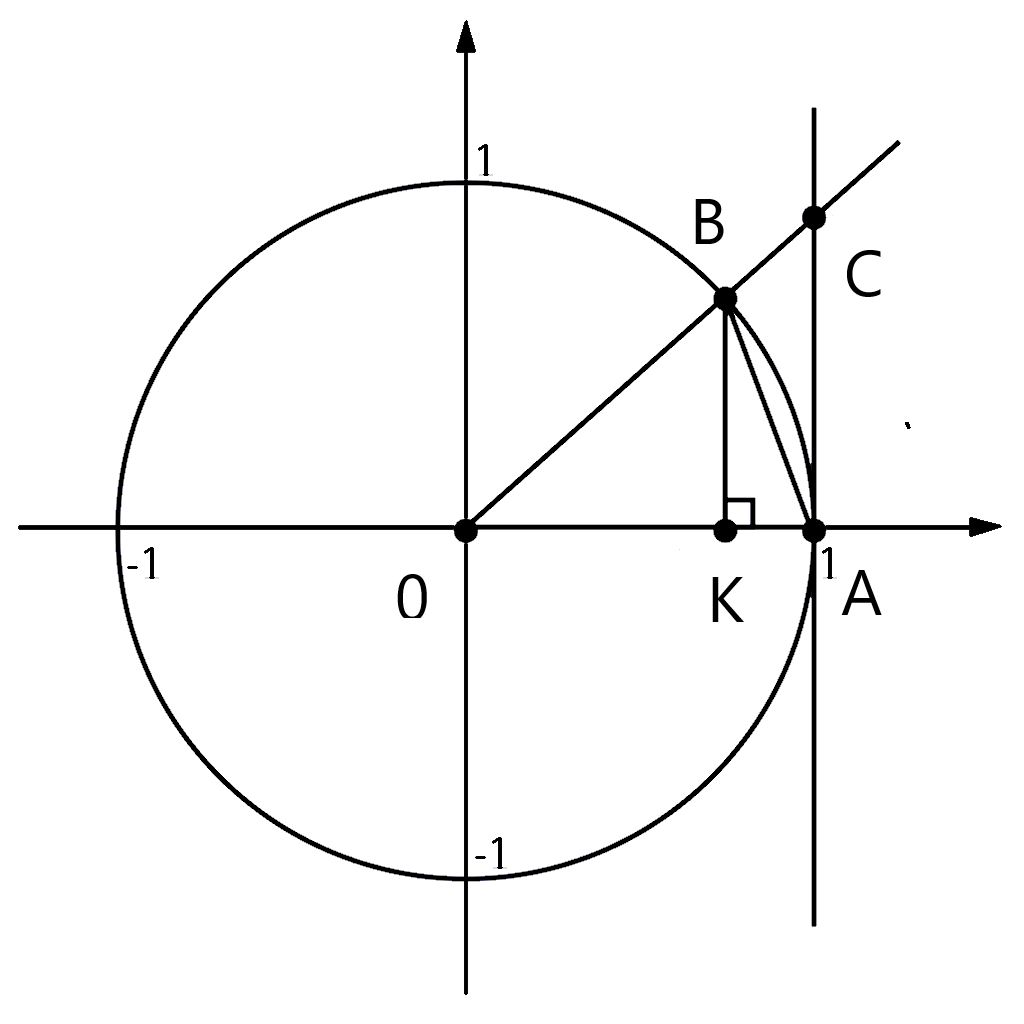
\includegraphics[scale=0.2]{image.png}
\end{wrapfigure}

Рассмотрим $\triangle$ DAB, $\triangle$ DAC и сектор OAB.
x-длинна дуги.
При $x \rightarrow 0$ их S уменьшаются.


$$ S\triangle{OBA} = \frac{1}{2}OA \cdot BK = \frac{\sin(x)}{2}$$
$$ S\triangle{OCA} = \frac{1}{2}OA \cdot AC = \frac{\operatorname{tg}(x)}{2}$$
$$ S(OBA) = \frac{1}{2}x \cdot r = \frac{x}{2}.$$

т.к. $ S\triangle OBA < SOBA < SOCA$
$\sin(x) < x < \operatorname{tg}(x)$

  $1  < \frac{x}{\sin(x)} < \frac{1}{\cos(x)}$

  $1 > \frac{\sin(x)}{x} > \cos(x)$

  это неравенство верно $\forall (x: 0 < |x|<\frac{\pi}{2})$.

  Функция, предел которой надо найти лежит между двумя функциями:
   $$\forall(\epsilon>0)\exists(\beta>0)\forall(x \in \mathbb{R})[0 < |x| <\beta \Rightarrow |\cos(x) - 1| < \epsilon]$$
  $$|\cos(x) - 1| = |2\sin^2(\frac{X}{2})| \leq 2|\sin\frac{x}{2}| < \frac{2|x|}{2} = |x| < \epsilon.$$

  Мы нашли $\beta : \beta = \epsilon$, т.к. |x| < $\beta$ и |x| < $\epsilon$. Получается:
  $$\lim\limits_{x\rightarrow 0}1=1, \lim\limits_{x \rightarrow 0}\cos(x) = 1
  \Rightarrow \lim\limits_{x \rightarrow 0}\frac{\sin(x)}{x}=1.$$

\subsection{Второй замечательный предел}
	\opred
	$\lim\limits_{x\rightarrow 0}(1+x)^\frac{1}{x}=e$ (1).
	\\
	$\lim\limits_{x\rightarrow \infty}(1+\frac{1}{x})^x=e$ (2).
	\subsubsection{Доказательство}
	$\lim\limits_{n\rightarrow \infty}(1+\frac{1}{n})^n=e$ - было ранее. Похоже на (2).
	Разница в том, что там - последовательность, а в (2) - просто числа.
	
	Воспользуемся теоремой о существовании и равенстве $\lim\limits_{x\rightarrow a\pm 0}$. Берем определение по Гейне.
	
	Рассмотрим 2 последовательность: $x_n и x_n^{'}: x_n \rightarrow 0 + 0; x_n^{'} \rightarrow 0-0$. 
	
	Надо показать, что $f(x)\rightarrow e$ слева и справа:
	Пусть $m_n =  [\frac{1}{x_n}]$; тогда $m_n \leq \frac{1}{x_n} \leq m_n + 1$.
	
	$$\frac{1}{m_n} \geq x_n \geq \frac{1}{m_n + 1} \bigg| +1$$
	$$ 1 + \frac{1}{m_n} \geq x_n + 1 \geq \frac{1}{m_n + 1} + 1$$
	$$\left(1 + \frac{1}{m_n}\right)^{m_n+1} \geq (x_n + 1)^{\frac{1}{x_n}} \geq \left(\frac{1}{m_n + 1} + 1\right)^{m_n+1}$$
	$$\left(1 + \frac{1}{m_n}\right)\left(1 + \frac{1}{m_n}\right)^{m_n} \geq (x_n + 1)^{\frac{1}{x_n}} \geq \left(\frac{1}{m_n + 1} + 1\right)^{m_n+1}
	\bigg| \left(\frac{1}{m_n + 1} + 1\right).$$
	
	Пусть $m_n \rightarrow \infty$.
	Тогда $\lim\limits_{m_n\rightarrow\infty}\left(1+\frac{1}{m_n}\right)\left(1+\frac{1}{m_n}\right)^{m_n}=e$, 
	$\lim\limits_{x\rightarrow\infty}\frac{\left(\frac{1}{m_n + 1} + 1\right)^{m_n+1}}{\frac{1}{m_n + 1} + 1}=e$
	$\bigg| \Rightarrow \lim\limits_{m_n\rightarrow\infty}(x_n + 1)^{\frac{1}{x_n}}=e$
	
	Это мы доказал стремление справа. Теперь докажем схождение слева. Пусть $x_n^{'} \rightarrow 0-0$ и 
	$x_n = \frac{-x_n^{'}}{1+x_n^{'}}$. Отсюда $x_n^{'}$ = $\frac{-x_n}{1+x_n}$.
	
	Значит, $f(x)=(1+x_n^{'})^{\frac{1}{x_n^{'}}}$=$\left(1 - \frac{x_n}{1+x_n}\right)^\frac{1+x_n}{-x_n}$=
	$\left(\frac{1+x_n-x_n}{1+x_n}\right)^{-\frac{1+x_n}{x_n}}=(1+x_n)^{\frac{1+x_n}{x_n}}=
	(1+x_n)^{1+\frac{1}{x_n}}=(1+x_n)(1+x_n)^{\frac{1}{x_n}}$.
	
	$\lim\limits_{x_n\rightarrow0}f(x)=\lim\limits_{x_n^{'}\rightarrow0-0}(1+x_n^{'})^{\frac{1}{x_n}}=e$.
	
	

 
\subsection{Бесконечно малые функции и их классификация}
\opred
	$f(x)$ - бесконечно малая функция, если $\lim\limits_{x\rightarrow0}f(x)=0$.

	\subsubsection {Утверждения, касающиеся бесконечно малых функций:}
	\begin{enumerate}
		\item $\lim\limits_{x\rightarrow0}f(x)=b \Leftrightarrow \lim\limits_{x\rightarrow0}(f(x)-b)-0$.

	     т.е. функкция $\alpha(x)=f(x)$ - бесконечно малая при $x \rightarrow a$.

		\item Сумма и произведение бесконечно малых функий при $x \rightarrow a$ есть бесконечно малая функции при $x \rightarrow a$.

		\item Произведение бесконечно малой функции при $x \rightarrow a$ на ограниченную функцию = бесконечно малая функция при $x \rightarrow a$.

		\end{enumerate}

	\subsubsection {Доказательство:}

	Пусть $f(x)$ - бесконечно малая, т.е. $\lim f(x)=0$. Пусть $g(x)$ - ограничена, т.е.
	$\exists(M>0)[|f(x)| \leq M]$ $|f(x)\cdot g(x)| \leq |f(x)|\cdot M$.

	$\lim\limits_{x\rightarrow a}(|f(x)||g(x)|)=\lim\limits_{x\rightarrow a}f(x) \cdot \lim\limits_{x\rightarrow a}M = 0 \cdot M = 0$.


	\subsubsection {Сравнение бесконечено малых функций.}

	Пусть есть $g(x) и f(x)$: X $\Rightarrow \ \mathbb {R}; X \subset  \mathbb {R}, x \rightarrow a$.

	$g(x) и f(x)$ - бесконечно малая одного порядка, если $$\lim\limits_{x\rightarrow a}\frac{g(x)}{f(x)}=b, (где b\neq 0).$$

	Бесконечно малые функции эквивалентны если $\lim\limits_{x \rightarrow 0}\frac{g(x)}{f(x)}=1$. Пишут: $g(x) \sim f(x)$.

	Например: $\sin(x) \sim x$.

	$f(x)$ - бесконечно малая функция высшего порядка малости по сравнению с g(x), если $\lim\limits_{x \rightarrow a}\frac{g(x)}{f(x)}=0$. Пишут: $f(x) = 0(g(x))$.

	Например: $x^2 = 0(x), при x \rightarrow 0$.

	\subsubsection {Теорема.}
	$f(x) \sim g(x) при x \rightarrow 0 \Leftrightarrow f(x) = g(x) = 0(f(x)) = 0(g(x))$

	\subsubsection {Доказательство:}

	$$\lim\limits_{x \rightarrow a}\frac{f(x) - g(x)}{f(x)} = \lim\limits_{x \rightarrow a}\left(1 - \frac{g(x)}{f(x)}\right) =
	 \lim\limits_{x \rightarrow a}1 - \lim\limits_{x \rightarrow a}\frac{g(x)}{f(x)0}=0$$

	$$\lim\limits_{x \rightarrow a}\frac{f(x) - g(x)}{g(x)} = \lim\limits_{x \rightarrow a}\left(\frac{g(x)}{f(x)} - 1\right) =
	 1 - \lim\limits_{x \rightarrow a}\frac{f(x)}{g(x)0}=0.$$

	чтд.

	$f(x) и g(x)$ - несравнимые бесконечно малые функции, если $$\not\exists \lim\limits_{x \rightarrow a}\frac{f(x)}{g(x)}.$$

	Например: $$f(x) = x\sin(\frac{1}{x}), g(x)=x, x\rightarrow 0: \lim\limits_{x \rightarrow 0}\frac{x\sin(\frac{1}{x})}x =
	 \lim\limits_{x \rightarrow 0}\sin(\frac{1}{x}) = \emptyset.$$

	$f(x) - бесконечно малая функция порядка k по сравнению с g(x), если \lim\limits_{x\rightarrow a}\frac{f(x)}{(g(x))^k}=b (b \neq 0)$

	Здесь $(g(x))^k$ - главня часть функции $f(x)$ по сравнению с $g(x)$.

	Например: $$\sin^{\lambda}x=f(x), g(x)=x, x=0, \lim\limits_{x \rightarrow 0}\frac{\sin^{2}x}{x^2}=1.$$

	Значит, $\sin^{2}x$ - функция порядка 2 по сравнению с $x, x^2$ - главная часть $\sin^{2}x$.

	\subsubsection {Теорема.}

	Пусть $g(x) \sim f(x) и f(x), g(x) бесконечно малая. Тогда \lim(f(x)\alpha(x))=\lim(g(x)\alpha(x))$, где $\alpha(x)$ - произвольная функция.

	\subsubsection {Доказательство:}

	$\lim(f(x)\alpha(x)) = \lim\frac{f(x)}{g(x)}g(x)\alpha(x) = \lim\frac{f(x)}{g(x)} \lim((g(x)) \alpha(x)) = \lim(g(x)\alpha(x))$.

	чтд.
\\
	Эта теорема позволяет сокращать вычисление $\lim$: некоторые множетили можно заменить эквивалентными.

	Например: $\lim\frac{\sin^{3}(x)}{x^3}=\lim\frac{x^3}{x^3}=1$.


\section{Непрерывные функции. Общие свойства}
\subsection{Понятие непрерывности функции в точке}
\subsubsection{Определение непрерывности функиции в точке по Коши.}

\opred

\fXR, $x_0 \in X$.
Функция $f$ непрерывна в точке $x_0$, если
$$
\forall(\epsilon>0)\exists(\delta>0)[|x-x_0|<\delta \Rightarrow |f(x)-f(x_0)|<\epsilon].
$$

Или, что то же самое, но с применением окрестностей:

$$
\forall(\epsilon>0)\exists(\delta>0) [f(U_{\delta}(x_0) \cap X) \subset U_{\epsilon}(f(x_0))]
$$

Или, что то же самое:

$$
\forall(\epsilon>0)\exists(\delta>0) [f(U_{\delta,X}(x_0)) \subset U_{\epsilon}(f(x_0))]
$$

И, наконец, полностью перейдя в термины окрестностей:

$$
\forall(U \in O(f(x_0)))\exists(V \in O_X(x_0)) [f(V) \subset U]
$$

\subsubsection{Замечание 1.}

Вдумчивый читатель легко заметит, что это определение похоже на определение предела в точке, в котором проколотые окрестности заменены на непроколотые. Несколькими строками ниже мы рассмотрим вопрос о связи непрерывности функции, её предела и её значения в данной точке.

\subsubsection{Замечание 2.}

Если $x_0$ - изолированная точка множества $X$, то
$$
 \exists(U \in O(x_0))[U \cap X = \{x_0\}] \Rightarrow f(U)=\{f(x_0)\}],
$$
т. е. найдётся окрестность точки $x_0$, образом которой явялется единственная точка, и функция $f$ в точке $x_0$ непрерывно. Однако никаких содержательных результатов этот случай не даёт, и потому в дальнейшем мы, как правило, будем рассматривать непрерывность функции, заданной на множестве точек, лишь в предельных точках этого множества.

\subsubsection{Критерий непрерывности функции в точке.}

\fXRx.
$f$ непрерывна в $x_0$ тогда и только тогда, когда 

$$
\lim_{x\to x_0}f(x)=f(x_0)
$$

\subsubsection{Следствие 1.}

\fXRx.
$f$ непрерывна в $x_0$ тогда и только тогда, когда знак предела и знак функции коммутируют, т. е. 
$$
\lim_{x \to x_0} f(x) = f(\lim_{x \to x_0}x)
$$

\subsubsection{Следствие 2.}

\fXRx, $f$ непрерывна в $x_0$, $\Delta y = f(x_0+\Delta x)-f(x_0)$.
$\Delta x \to 0$ тогда и только тогда, когда $\Delta y \to 0$

\subsubsection{Определение непрерывности в точке по Гейне.}

\fXRx.
$f$ непрерывна в $x_0$, если 
$$
\forall(\{x_n\}:x_n \in X \cap x_n \to x_0)[f(x_n)\to f(x_0)]
$$

Обозначив $\Delta x = x_n-x_0$, $\Delta x = f(x_n)-f(x_0)$, можем сформулировать:

$$
\Delta x \to 0 \Rightarrow \Delta y \to 0
$$


\subsection{Непрерывность функции на множестве}
\opred

Функция $f:X\to \R$ называется непрерывной на $X$, если она непрерывна во всех точках $x \in X$.

\opred

Если функция $f:x \to \R$ не является непрерывной в точке $x_0 \in X$, то $x_0$ называется точкой разрыва функции $f$.

\subsubsection{Замечание 1.}

Так как все точки множества $\N$ изолированны, то любая функция $f:\N \to \R$ непрерывна.

\subsection{Понятие колебания функции на множестве и в точке. Необходимое и достаточное условие непрерывности функции в точке}
\opred

\fXR, $E \subset X$, $\alpha_E=\inf_E f(x)$, $\beta_E=\sup_E f(x)$.
Тогда разность $\alpha_E-\beta_E$ называется колебанием функции $f$ на множестве $E$:

$$
\omega(f,E)=\alpha_E-\beta_E=\sup_E f(x) - \inf_E f(x)
$$

Или, что то же самое, 

$$
\omega(f,E)=\sup_{a,b \in E}(f(a)-f(b))
$$

\subsubsection{Примеры.}

$\omega(x^2,[-2;4])=16$

$\omega(\sgn x,[0;4])=1$

$\omega(\sgn x,(0;4])=0$

$\omega(\sgn x,[-1;4])=2$

\opred

\fXRx.
Величина $\lim_{\delta \to 0+}\omega(f,U_{\delta}(x_0))$ называется колебанием функции $f$ в точке $x_0$:

$$
\omega(f,x_0)=\lim_{\delta \to 0+}\omega(f,U_{\delta}(x_0))
$$

\subsubsection{Теорема.}

Пусть $f:X\to\R$.
Функция $f$ непрерывна в точке $x_0\in X$ тогда и только тогда, когда $\omega(f,x_0)=0$.

\subsection{Односторонняя непрерывность}
\opred
	Пусть $x_0 \in x$. Функция f(x) непрерывна в $x_0$ справа, если: $$\forall(\epsilon>0)\exists(\beta>0)\forall(x \in X)[x_0 < x < x_0+\beta\rightarrow |f(x)-f(x_0)| < \epsilon]$$

	непрерывна слева, если:  $$\forall(\epsilon>0)\exists(\beta>0)\forall(x \in X)[x_0 - \beta < x < x_0\rightarrow |f(x)-f(x_0)| < \epsilon]$$

\subsubsection{Утверждение 1.}
	Сравнивая это определение с определением правого(левого) $\lim f(x)$ по Коши, легко доказать, что справедливо утверждение 1:
	Если $x\rightarrow x_0 + 0$ $(x_0-0)$, то f(x) - непрерывная справа(слева) $\leftrightarrow\lim\limits_{x\rightarrow x_0\pm0}=f(x_0)$.

\opred
	Функця f(x) - непрерывна справа(слева) в $x_0$, если $$\forall({x_n}:x_n\subset X\wedge x_n \rightarrow x_0 \pm0 )[f(x_n)\rightarrow f(x_0)]$$

\subsubsection{Утверждение 2.}f(x) неперывна в $x_0 \in X \leftrightarrow f(x)$ - непрерывна справа и слева в этой точке $x_0$.

\opred
	Функция разрывна в $x_0$ справа(слева), если она не непрерывна справа(слева).

\subsubsection{Упражнение} Доказать, что f(x) = [x] - непрерывна справа в $\forall$ целой точке и разрывна слева в этой точке. А в $\forall$ точке x $(x\notin \mathbb {Z})$ она неперрывна справа и слева, т.е просто непрерывна.

\subsection{Классификация точек разрыва}
\opred
Точки разрыва функций $f(x)$ - точки множества $X$, в которых $f(x)$ разрывна.

Наряду с точками, принадлежащими $D(f)$, будем рассматривать и те точки, в которых $f(x)$ неопределена, но которые являются предельными для для области определения $f(x)$.

Например для $f(x)=\frac{1}{x}$ рассматриваем и $x=0$.

Типы разрыва:

\opred
1) Устранимый разрыв.

Пусть $x \to x_0$ , $x_0$ - точка устранимого разрыва функции $f(x)$, если 

$\exists (\lim_{x \to x_0} f(x) = b)$, $b \neq \infty$, но в $x_0$ $f(x)$ либо неопределено, либо

$f(x_0) = a, a \neq b$.

\subsubsection{Пример}
a) $f(x) = \frac{sin x}{x}$, $x_0$ точка устранимого разрыва, т.к. $\lim_{} f(x) = 1$, а 

$x=0\notin D(f)$. Функция неопределена в $x=0$, но $\exists (\lim_{} f(x) = 1)$.

Значит, этот $x=0$ мы можем "внести" в график, чуть изменив условие:

б)
\begin{equation*}
f(x) = 
 \begin{cases}
   \frac{sin x}{x} &\text{$x \neq 0$}\\
   1 &\text{$x = 0$}
 \end{cases}
\end{equation*}
Теперь

$$\lim_{x \to 0}\frac{sin x}{x} = 1 =\lim_{x \to 0} f(x)$$

2) Разрыв первого рода (конечный скачок).

\opred
$x_0$ - точка разрыва первого рода, если:
$$a=\lim_{x \to x_0 + 0} f(x) \neq \lim_{x \to x_0 - 0} f(x)$$

\subsubsection{Например}
а)
$$f(x) = sign x$$
$$\lim_{x \to + 0} f(x) = 1$$
$$\lim_{x \to - 0} f(x) = -1$$
$$1 \neq -1$$

\subsubsection{Например}
б)
$$f(x) = \frac{sin x}{|x|}$$
$$\lim_{x \to x_0 + 0} f(x) = 1$$
$$\lim_{x \to x_0 - 0} f(x) = -1$$
$\lim_{x \to x_0 \pm  0} f(x)$ - существуют, но не равны.

3) Разрыв второго рода.

\opred
$x_0$ - точка разрыва первого рода, если в $x_0$ $f(x)$ не имеет хотя бы один $\lim_{x \to x_0 \pm  0}$ или один из них $\infty$

\subsubsection{Например}
а) $f(x) = sin \frac {1}{x}$ при $x=0$ - $\lim$ нет ни +0, ни -0

б)$f(x) = 3^\frac{1}{x} - \lim_{x \to x_0 + 0} = +\infty$
\subsection{Локальные свойства непрерывных функций}
...

\section{Функции, непрерывные на отрезке}
\subsection{Теорема Больцано-Коши и следствия из неё}
\subsubsection{Теорема.}
Пусть $f:[a;b]\to \R$ и $f$ непрерывна на $[a;b]$, при этом $f(a) \cdot f(b) <0$,
т. е. на концах отрезка $[a;b]$ непрерывная на нём функция $f$ принимает значения разного знака.
Тогда $\exists(c \in (a;b))[f(c)=0]$,
т. е. хотя бы в одной точке интервала $(a;b)$ функция обращается в нуль.

\subsubsection{Замечание.}
Теорема Больцано-Коши не только утверждает существование точки, в которой функция обращается в нуль, но и фактически даёт способ её найти - методом половинного деления отрезка. Этот факт может быть применён при нахождении корня уравнения численными методами.

\subsubsection{Следствие 1 (теорема о промежуточном значении).}
\fXR, при этом $f$ непрерывна на некотором промежутке $Y \subset X$, $\{a;b\}\subset Y$, $a<b$.
Тогда $\forall(\gamma$ между $f(a)$ и $f(b))\exists(c:c\in[a;b])[f(c)=\gamma]$.

\subsubsection{Следствие 2.}
\fXR, $X$ - промежуток и $f$ непрерывна на нём.
Тогда $f(X)$ - тоже промежуток.


 


\subsection{Первая теорема Вейерштрасса}
\subsubsection{Теорема.}

Функция, непрерывная на отрезке, ограничена на нём.

\opred

Компактом (компактным множеством) называется такое множество $X$, что
$$
\forall(\{x_n\}:x_n \in X)\exists(\{x_{n_k}\})[\{x_{n_k}\}\to x_0 \in X],
$$ 
т. е. в любой последовательности точек этого множества можно выделить подпоследовательность, сходящуюся к точке этого множества.

\subsubsection{Замечание.}
Конечный или бесконечный интервал $(a;b)$, где $\{a;b\}\subset\overline\R$, не является компактом, т. к. любая подпоследовательность любой последовательности его точек, сходящейся к $a$ или $b$, сходится к не принадлежащей интервалу точке $a$ или $b$ соответственно.

Полуинтервал также не является компактом.
Предоставляем читателю доказать это самостоятельно.

\subsubsection{Обобщение первой теоремы Вейерштрасса.}

Функция, непрерывная на компакте, ограничена на нём.

\subsubsection{Замечание.}

Функция, определённая на некомпактном множестве, может быть на нём неограничена. Пример - тождественная функция $f(x)=x$ на некомпактом множестве $(-\infty;+\infty)$.


\subsection{Вторая теорема Вейерштрасса}
\subsubsection{Теорема.}

Функция, непрерывная на компакте, достигает на нём точных верхней и нижней границ множества своих значений.

\mnemo
Эту теорему можно запоминать по начертанию цифры {\LARGE 2}, разделив его на три части: горизонтальная черта снизу - отрезок, средняя часть - непрерывная функция, <<завиток>> сверху - точное верхнее значение.


\subsubsection{Следствие.}

Пусть $f:[a;b]\to\R$ и $f$ непрерывна, $\alpha=\inf(f[a;b])$, $\beta=\sup(f[a;b])$.
Тогда $f([a;b])=[f(a);f(b)]$.




\subsection{Понятие равномерной непрерывности функции. Теорема Кантора, следствия из неё}
Согласно определению непрерывности,
$f:X \to R$ непрерывна, если 
$\forall(x_0 \in X) \forall(\epsilon >0) \exists(\delta>0)[0<|x-x_0|<\delta \Rightarrow |f(x)-f(x_0)|<\epsilon] $

В общем случае $\delta$ зависит от $\epsilon$ и $x_0$, т. е. $\delta=\delta(\epsilon,x_0)$.
Однако иногда $\delta$ зависит только от $\epsilon$ и не зависит от $x_0$, т. е. $\delta=\delta(\epsilon)$.

\opred
$f(x)$ равномерно непрерывна на $X$, если
$$ \forall(\epsilon >0) \exists(\delta>0) \forall(x_0 \in X) [0<|x-x_0|<\delta \Rightarrow |f(x)-f(x_0)|<\epsilon] $$

\subsubsection{Замечание 1.}
Если $f(x)$ равномерно непрерывна на $X$, то $f(x)$ непрерывна на $X$.
(Т.~к. квантор общности $\forall$ можно переносить вправо.)

\subsubsection{Замечание 2.}
Не всякая функция $f$, непрерывная на $X$, равномерно непрерывна на $X$.
(Например: $f(x)=x^2, f:\R \to \R$.)


\subsubsection{Теорема Кантора о равномерной непрерывности.}
\fXR, $X$ - компакт и $f$ непрерывна на $X$.
Тогда $f$ равномерно непрерывна на $X$.

\subsubsection{Следствие 1.}

Если $f:[a;b] \to \R$ непрерывна на отрезке $[a;b]$, то она равномерно непрерывна на этом отрезке.

\subsubsection{Следствие 2.}

Если $f:[a;b] \to \R$ непрерывна на отрезке $[a;b]$, то
$$
\forall(\epsilon > 0) \exists (\delta > 0) \exists(a_1, b_1 : a < a_1 < b_1 < b, b_1 - a_1<\delta)[\omega(f,[a_1,b_1]<\epsilon],
$$
или, что то же самое,
$$
\forall(\epsilon > 0) \exists (отрезок \Delta \subset [a;b])[\omega(f,\Delta)<\epsilon]
$$
т. е. найдётся подотрезок, на котором колебание функции меньше любого наперёд заданного.

\subsubsection{Замечание.}



\subsection{Свойства монотонных функций. Теорема об обратной функции}
\subsubsection{Лемма 1.}

Непрерывная функция, заданная на отрезке, инъективна в том и только том случае, когда она строго монотонна.

\subsubsection{Лемма 2.}

Пусть $X \subset \mathbb{R}$.
Любая строго монотонная функция $f:X \to Y \subset \mathbb{R}$ обладает обратной функцией $f^{-1}:Y \to X$,
причём обратная функция $f^{-1}$ имеет тот же характер монотонности на $Y$, что и функция $f$ на $X$.

\subsubsection{Лемма 3.}

Пусть $X \subset \mathbb{R}$.
Монотонная функция $f:X\to \mathbb{R}$ может иметь разрывы только первого рода.

\subsubsection{Следствие 1.}

Если $a$ - точка разрыва монотонной функции $f$, то по крайней мере один из пределов функции $f$ слева или справа от $a$ определён.

\dokvo

Если $a$ - точка разрыва, то она является предельной точкой множества $X$ и, по лемме 3, точкой разрыва первого рода.
Таким образом, точка $a$ является по крайней мере правосторонней или левосторонней предельной для множества $X$, т. е. выполнено хотя бы одно из следующих условий:
\[
f(a-0)=\lim_{x \to a-0}f(x)
\]
\[
f(a+0)=\lim_{x \to a+0}f(x)
\]
Если $a$ - двусторонняя предельная точка, то существуют и конечны оба односторонних предела.

\subsubsection{Следствие 2.}

Если $a$ - точка разрыва монотонной функции $f$, то по крайней мере в одном из неравенств $f(a-0)\leq f(a)\leq f(a+0)$ - для неубывающей $f$ или $f(a-0)\geq f(a)\geq f(a+0)$ - для невозрастающей $f$, имеет место знак строгого неравенства, т. е. $f(a-0) < f(a+0)$ - для неубывающей $f$ или $f(a-0) > f(a+0)$ - для невозрастающей $f$, и в интервале, определённым этим строгим неравенством, нет ни одного значения функции.
(Также говорят: интервал свободен от значений функции.)

\subsubsection{Следствие 3.}

Интервалы, свободные от значений монотонной функции, соответствующие разным точкам разрыва этой функции, не пересекаются.

\subsubsection{Лемма 4. Критерий непрерывности монотонной функции.}

Пусть даны отрезок $X=[a;b] \subset \mathbb{R}$ и монотонная функция $f:X \to \mathbb{R}$.
$f$ непрерывна в том и только том случае, когда $f(X)$ - отрезок $Y$ с концами $f(a)$ и $а(b)$.
($f(a) \leq f(b)$ для неубывающей $f$, $f(a) \geq f(b)$ для невозрастающей $f$).

\dokvo
\neobh

Т. к. $f$ монотонна, то все её значения лежат между $f(a)$ и $f(b)$. Т. к. $f$ непрерывна, то она принимает и все промежуточные значения. Следовательно, $f(X)$ - отрезок.

\dost

\pp, т. е. что $\exists \left(c \in [a;b]\right)$ - точка разрыва $f$.
Тогда по следствию 2 леммы 3 один из интервалов: $\left(f(c-0);f(c)\right)$ или $\left(f(c);f(c+0)\right)$ - определён и не содержит значений $f$.
С другой стороны, этот интервал содержится в $Y$, т. е. $f$ принимает не все значения из $Y$, $f(X)\neq Y$. Получили противоречие.












\subsubsection{Теорема.}
\fXR и $f$ строго монотонна.
Тогда существует обратная функция $f^{-1}:Y \to X$, где $Y=f(X)$, притом $f^{-1}$ строго монотонна на $Y$ и имеет тот же характер монотонности, что и $f$ на $X$.
Если, кроме того, $X=[a;b]$ и $f$ непрерывна на отрезке $X$, то $f([a; b])$ есть отрезок с концами $f(a)$ и $f(b)$ и $f^{-1}$ непрерывна на нём.


\subsection{Непрерывность элементарных функций}
1) Показательная функция. 

$y=a^x$, $(a>1)$ монотонно $\nearrow$ в промежутке $X=(-\infty;+\infty)$.
Ее значения $>0$ и заполняют весь промежуток $Y=(0;+\infty)$. Это видно из $\exists (x=log_a y)\forall (y>0)$, следовательно $f(x)$ непрерывна $\forall(x \in X)$.

2) Логарифмическая функция. 

$y=log_a x (a>0, a \neq 1)$.
Пусть $a>1$, тогда $f(x)\nearrow$ при $x \in X = (0; +\infty)$. К тому же, $f(x)$ принимает любое значение из $(-\infty;+\infty)$, следовательно $f(x)$ непрерывна.

3) Степенная функция. 

$y=x^\alpha (\alpha \neq 0)$

При $x: (0; +\infty)$

$f(x)\nearrow(\alpha > 0)$

$f(x) \searrow(\alpha < 0)$

$f(x) \in (0; +\infty)$

4) Тригонометрические функции.

$y = sin x$ - непрерывна на $X = [-\frac{\pi}{2};\frac{\pi}{2}]$ (т.к. $f(x)$ монотонна и принимает $\forall$ значений из $[-1;1]$). 

Также $f(x)$ - непрерывна на $ X = (k\pi - \frac{\pi}{2};k\pi + \frac{\pi}{2}) \forall (k \in \mathbb {Z})$.

Итого : $f(x)$ - непрерывна для $\forall (x)$.

Аналогично : $y=cos x$ непрерывна для $\forall (x)$.

Отсюда вытекает непрерывность :

$tg = \frac{sin x}{cos x}$, кроме $x = (2k + 1)\frac{\pi}{2}$,

$arctg = \frac{cos x}{sin x}$, кроме $x = k\pi$

$sec = \frac{1}{cos x}$, кроме $x = (2k + 1)\frac{\pi}{2}$,

$cos = \frac{1}{sin x}$, кроме $x = k\pi$.

5)Обратные тригонометрические функции.

$y = arcsin x, y = arccos x$ непрерывны на $[-1;1]$

$y = arctg x, y = arcctg x$ непрерывны на $[-\infty;+\infty]$



\chapter{Основы дифференциального исчисления}
\section{Дифференциальное исчисление функции одной независимой переменной}
\subsection{Определение производной и дифференциала, связь между этими понятиями}
\subsection{Связь между понятиями дифференцируемости и непрерывности функций}
\subsection{Дифференцирование и арифметические операции}
\subsection{Теорема о производной сложной функции. Инвариантность формы первого дифференциала}
\subsection{Теорема о производной обратной функции}
\subsection{Производные основных элементарных функций. Доказательство}
\subsection{Касательная к кривой. Геометрический смысл производной и дифференциала}
\subsection{Физический смысл производной и дифференциала}
\subsection{Односторонние и бесконечные производные}
\subsection{Производные и дифференциалы высших порядков}
...

\section{Основные теоремы дифференциального исчисления}
\subsection{Понятие о локальном экстремуме функции}
\opred

\fXRx.
Точка $x_0$ называется точкой локального минимума, а значение в ней - локальным минимумом функции $f$, если
$$
\exists (U(x_0)) \forall(x \in U(x_0) \cap X)[f(x) \geq f(x_0)]
$$

\opred

\fXRx.
Точка $x_0$ называется точкой локального максимума, а значение в ней - локальным максимумом функции $f$, если
$$
\exists (U(x_0)) \forall(x \in U(x_0) \cap X)[f(x) \leq f(x_0)]
$$

\opred

\fXRx.
Точка $x_0$ называется точкой строгого локального минимума, а значение в ней - строгим локальным минимумом функции $f$, если
$$
\exists (\mathring{U}(x_0)) \forall(x \in \mathring{U}(x_0) \cap X)[f(x) > f(x_0)]
$$

\opred

\fXRx.
Точка $x_0$ называется точкой строгого локального максимума, а значение в ней - строгим локальным максимумом функции $f$, если
$$
\exists (\mathring{U}(x_0)) \forall(x \in \mathring{U}(x_0) \cap X)[f(x) < f(x_0)]
$$

\opred

Точками локального экстремума называются вместе точки локального минимума или максимума.

\opred

Локальными экстремумами называются вместе локальные минимумы или максимумы.

\opred

Точками строгого локального экстремума называются вместе точки строгого локального минимума или максимума.

\opred

Строгими локальными экстремумами называются вместе строгие локальные минимумы или максимумы.

\opred

\fXR, $x_0$ - двусторонняя предельная точка $X$.
Если $x_0$ - точка локального экстремума, то она называается точкой внутреннего локального экстремума.



\subsection{Теорема Ферма}
\subsubsection{Теорема Ферма о производной в точке локального экстремума.}

\fXR, $f$ дифференцируема в точке внутреннего локального экстремума $x_0$.
Тогда $f'(x_0)=0$.

\subsubsection{Замечание 1.}

В невнутренней точке локального экстремума производная может, вообще говоря, быть не равной нулю.
Пример: $f:[-1;1]\to \R$, невнутренний локальный максимум $x_0 = 1$, $f'(x_0)=2$.

\subsubsection{Замечание 2.}
Теорема Ферма необратима.
Пример: $f:\R\to\R$, $f(x)=x^3$, $f'(0)=0$, но $f$ не имеет локальных экстремумов.




\subsection{Теорема Ролля}
\subsection{Теорема Лагранжа и следствия из нее}
\subsection{Теорема Коши}
...

\section{Формула Тейлора}
\subsection{Формула Тейлора для многочлена}
\subsection{Формула Тейлора для произвольной функции. Различные формы остаточного члена формулы Тейлора}
\subsection{Локальная формула Тейлора}
\subsection{Формула Маклорена. Разложение по формуле Маклорена некоторых элементарных функций}
...

\section{Правило Лопиталя}
Пусть даны две непрерывные на интервале $(a; b)$ функции $f(x)$ и $g(x)$, где $\{a; b\} \subset \overline{\mathbb{R}}$. Неопределённостью типа $\left[\frac{0}{0}\right]$ в точке $a$ называется предел 
\[
\lim_{x \to a+}\frac{f(x)}{g(x)}
\]
в случае, когда
\[
\lim_{x \to a+}f(x) = \lim_{x \to a+}g(x) = 0
\]
Аналогично определяются неопределённости вида $\left[\frac{\infty}{\infty}\right]$ и в точке $b$.

Другие виды неопределённостей сводятся к этим двум. Вообще говоря, неопределённость типа $\left[\frac{\infty}{\infty}\right]$ может быть сведена к типу $\left[\frac{0}{0}\right]$. Действительно, пусть
$\lim_{x \to a+}f(x) = \lim_{x \to a+}g(x) = \infty$
\[
\frac{f(x)}{g(x)}=\frac{\frac{f(x)}{g(x)}}{\frac{f(x)}{g(x)}}
\]
 






\end{document}
